% RESULTADOS PARA ANISOTROPÍAS EN RA PARA ALL TRIGGERS
  \section{Anisotropías en ascensión recta en los archivos con todos los disparos}
% ---> CARACTERISTICAS
    \subsection{Características de los archivos de datos analizados}

      Tenemos que tener en cuenta el archivo de datos de todos los disparos es entre los años 2013 y 2019, por lo que no podemos comparar los análisis de anisotropía con el conjunto  de datos del ICRC 2019 completo. %Por lo que para compararlos, voy a hacer el análisis de ambos conjuntos de datos en el mismo rango de tiempo. Voy a hacer esto para poder comparar lo que sale.       Este rango donde se está comparando entre archivo empieza en  $utc_i = 1372699409 $.

    %CARACTERISTICAS GENERALES DE AMBOS SET DE DATOS.

      A continuación se presentan las características de los archivos estudiados, sin ningún filtro de energía, sin acotar por tiempo. 

      \begin{table}[H]
      \centering
        \begin{tabular}{c|c|c|c}
        \textbf{Archivo} & \text{Eventos} & UTC inicial &  UTC final  \\ \hline
        2020       & 13 739 351   &  1372680068 &  1577879983 \\
        2019       &  8 463 063   &  1372680068 &  1496318388 \\
        2017       &  8 592 302   &  1372680068 &  1498521517 \\
          \end{tabular}
      \end{table}
      
      Puede verse que el Archivo de 2020 tiene más eventos, y además de tener un rango de tiempo mayor que el archivo del 2017 y 2019. Los archivos 2017 y 2019  tienen $7\,072\,964$ eventos coincidentes y los archivos 2017 y 2020 tienen $6\,902\,21$ A continuación se compara la diferencia de energía y la calibración entre estos eventos.

    %COMPARANDO DELTA E ENTRE LOS DOS ARCHIVOS
      En las  Figs.\,\ref{fig:deltaE} y \ref{fig:histograma} se muestra la diferencia entre el valor de energía entre eventos coincidentes entre los archivos 2017 y 2020. Puede apreciarse que la diferencia no esta centrada 0 y no aparenta tener una modulación del clima. Por lo tanto la diferencia se debe a una reconstrucción distinta de los eventos.

          \begin{figure}[H]
            \begin{subfigure}[b]{0.5\textwidth}
              \centering
              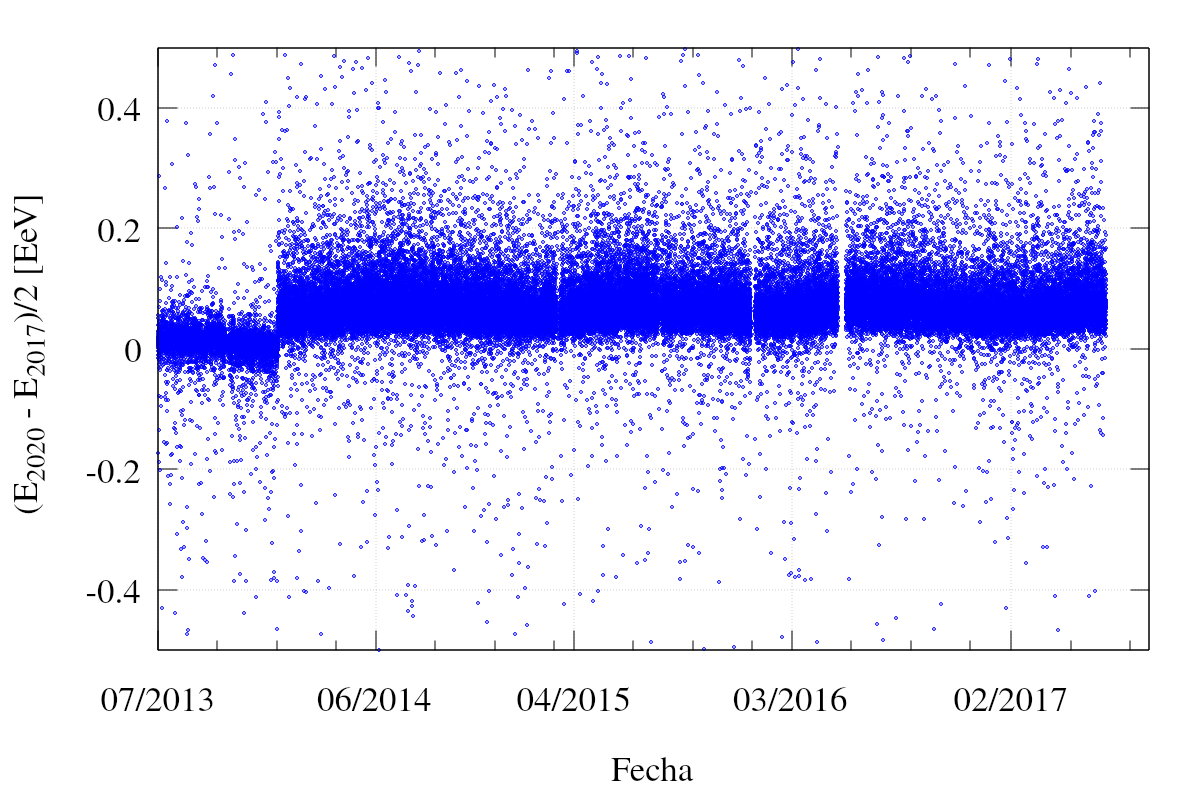
\includegraphics[width=\textwidth]{../0_Introduccion/comparacion_deltaE.png}
              \caption{Diferencia entre las energías} \label{fig:deltaE}
            \end{subfigure}%
            \begin{subfigure}[b]{0.5\textwidth}
              \centering
              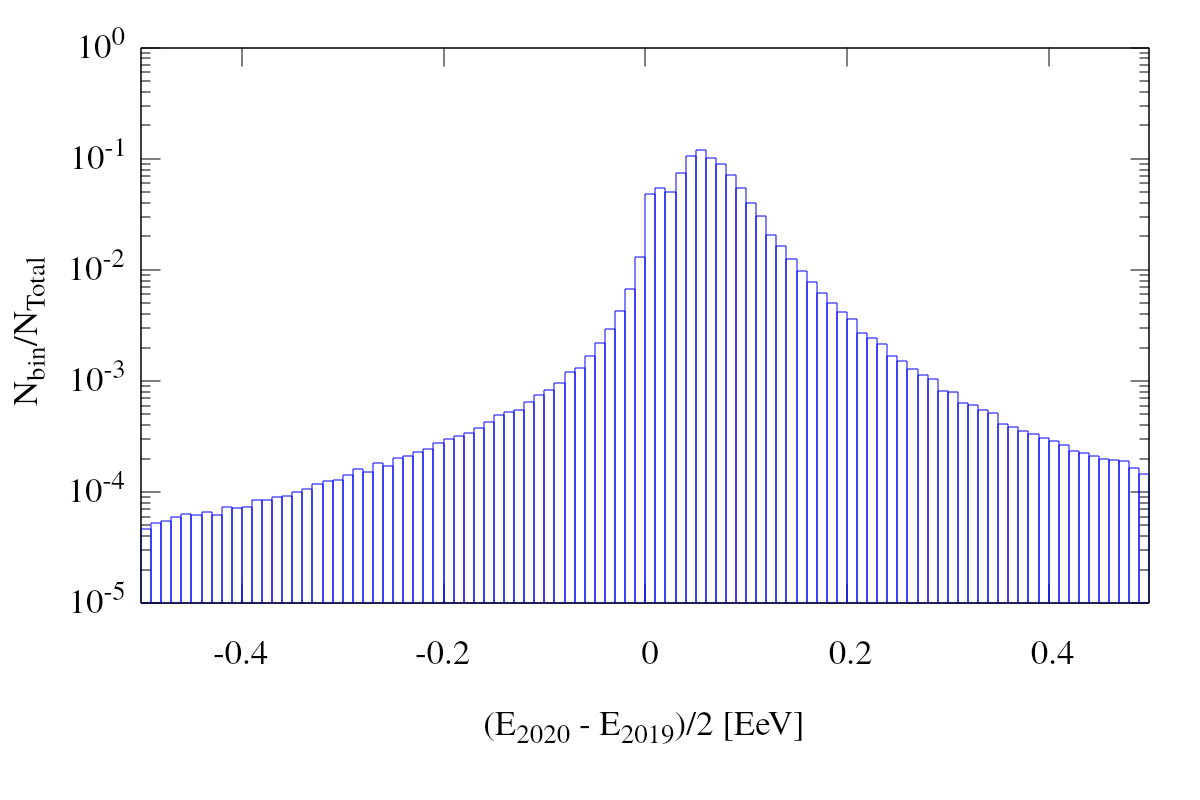
\includegraphics[width=0.8\textwidth]{../0_Introduccion/histograma_deltaE.png}
              \caption{Histograma de las diferencias}   \label{fig:histograma}
            \end{subfigure}
            \caption{Diferencia entre las energías del archivo de 2017 y el archivo del 2019}
          \end{figure}

    %COMPARANDO LA CURVA DE CALIBRACIÓN ENTRE LOS DOS ARCHIVOS
      Puede verse en la Fig.\,\ref{fig:calibracionE} que la curva de calibración entre ambos archivos es distinta, ya que la coordenada al origen como la pendiente es difieren entre para ambos archivos. Esto implica que los valores A y B de la curva $E=A\times (S_{38})^B$ son distintos para ambos conjunto de datos, ¿en qué afectaría? en primer lugar en el valor de la energía, segundo en análisis que dependan del estos parámetros como el análisis de la modulación del clima.

        \begin{figure}[H]
          \centering
          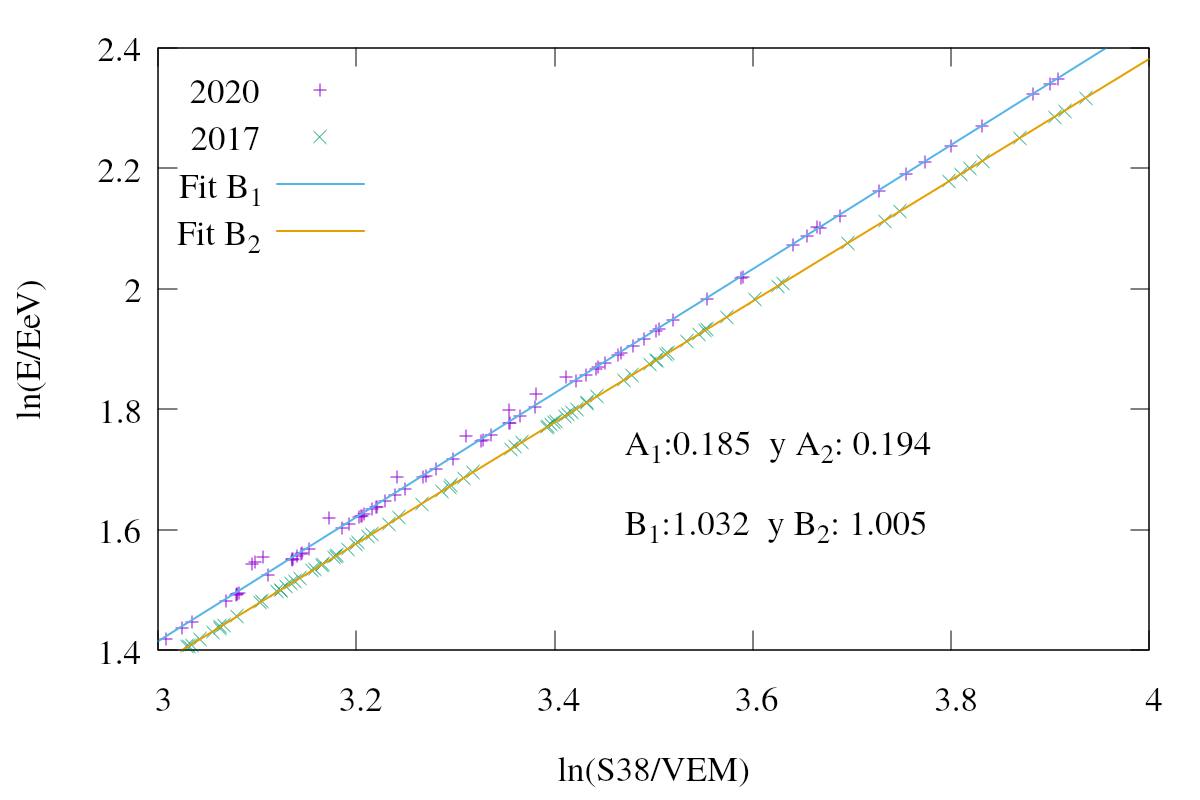
\includegraphics[width=0.65\textwidth]{../0_Introduccion/comparacion_reconstruccion.png}
          \caption{Calibración de las energías del archivo de 2017 y el archivo del 2019}
          \label{fig:calibracionE}
        \end{figure}
	
%%%%%%%%%%%%%%%555
%%%%%%%%%%%%%%%%%%
%%%%%%%%%%%%%%%%%5555555tttttttt




	\section{Características del conjunto de datos} \label{specs}
	

	Además de los filtros aplicados mencionados en la sección \ref{filtro}, se aplican filtros adicionales sobre la energía y el rango de tiempo. Para estudiar los eventos en esta sección, consideramos los eventos entre 1\,EeV y 2\,EeV de energía y que ocurrieron entre las 12:00:00 GMT del 1 de enero de 2013 y las 12:00:00 GMT del 1 de enero de 2020. Se  eligió ese rango de tiempo, ya que el registro de eventos más reciente al que se tuvo para hacer este trabajo termina el 1 de Enero del 2020  a las 11:59:43 GMT, además de para estudiar una cantidad entera de años, se optó por considerar los eventos desde el 1 de Enero del 2013 a las 12:00:00 GMT.

	Un resumen de todos los filtros aplicados se encuentra a continuación
		\begin{enumerate}
			\item Son eventos obtenidos mediante todos los disparos.
			\item Energía entre  [1 EeV , 2 EeV)
			\item Rango de tiempo:
			\begin{itemize}
				\item[-] Inicial:1388577600 (Jueves, 1 de Enero de 2014 12:00:00 GMT)
				\item[-] Final: 1577880000  (Jueves, 1 de Enero de 2020 12:00:00 GMT)
			\end{itemize}
			\item Ángulo cenital $\theta < 60^o$
			\item 6T5
			\item $ib=1$ Bad period flag. Un valor de 1 indica un buen periodo
		\end{enumerate}
	Aplicando estos filtros, se tienen $1\,081\,844$ eventos para estudiar en este rango de energía.
			
			\begin{figure}[H]
				\centering
				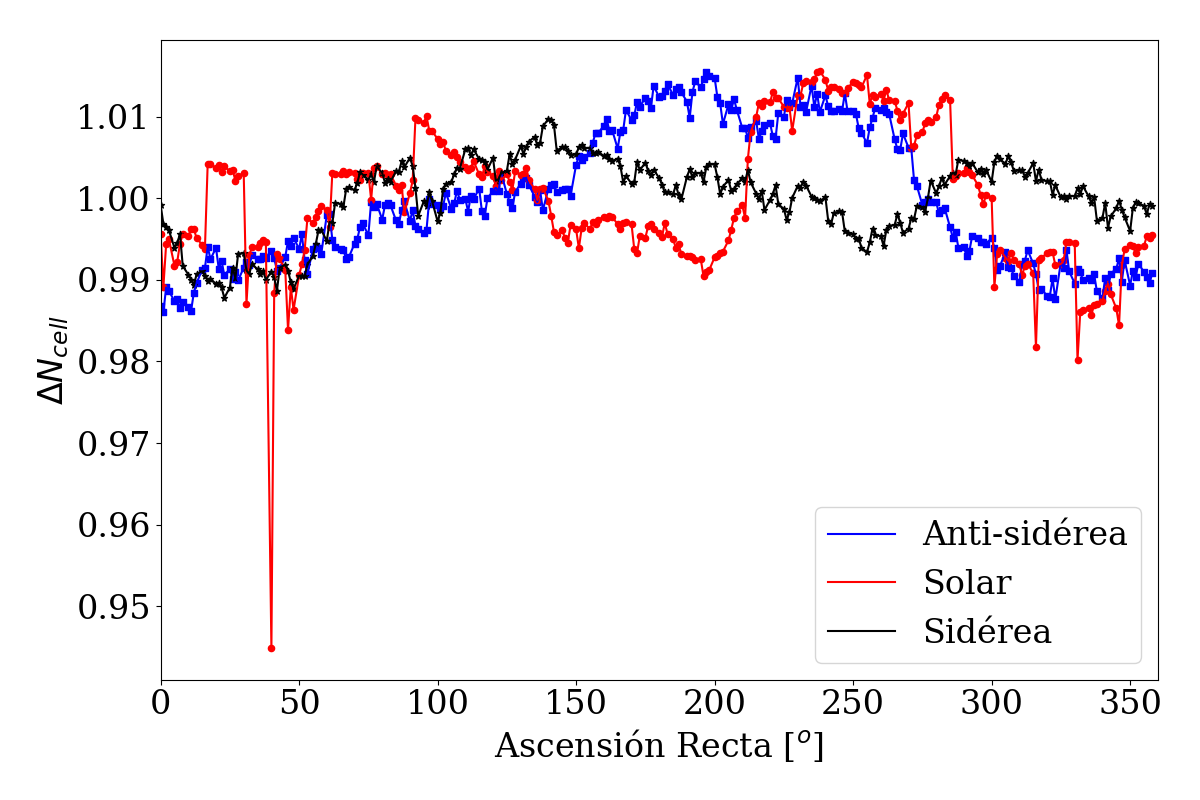
\includegraphics[width=0.75\textwidth]{weights_2013_2020.png}
				\caption{Variaciones de los hexágonos para frecuencias características en rango mencionado. }
			\end{figure}

\section{Pesos de los eventos para frecuencias de referencia}

Se toman las frecuencia anti-sidérea ($f_a=364.25\,$ciclos), solar ($f_{Solar}= 365.25\,$ciclos) y sidérea ($f_{sid}= 366.25\,$ciclos) como referencia para obtener una aproximación a primer orden del análisis en frecuencias. A cada una de estas frecuencias, se ajusta una función del tipo  $f(x)=a\cdot \cos{(\alpha-\phi)} + 1$, con el se busca aproximar la amplitud $a$ y el desfase $\phi$ de las curvas de los pesos en función de la ascensión recta $\alpha$. Los ajustes se observan en las Figs. \ref{fig:ajuste_antisiderea}, \ref{fig:ajuste_solar} y \ref{fig:ajuste_siderea}.


\subsection{Gráficos de los ajustes}


\begin{figure}[H]
\begin{subfigure}{.5\textwidth}
	\centering
	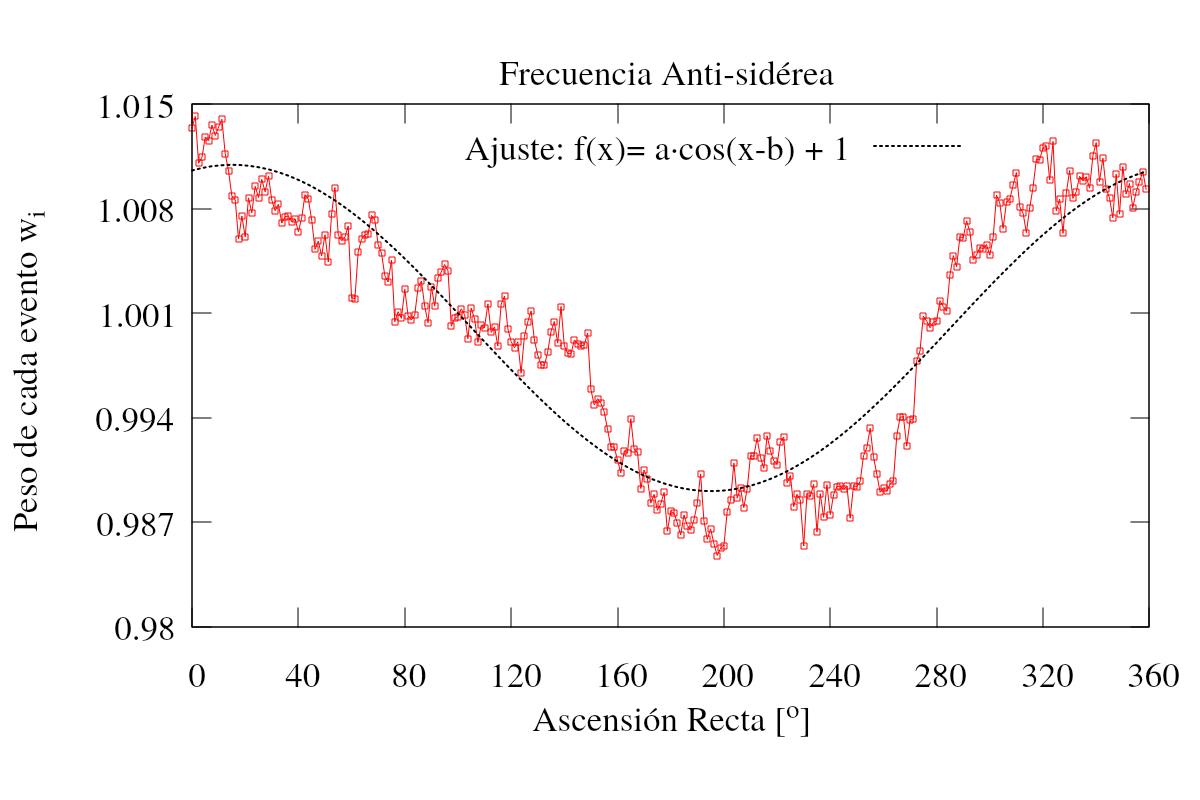
\includegraphics[width=\linewidth]{eventos_RA_ajuste_cos_antisiderea_v2.png}
	\caption{Frecuencia anti-sidérea}
	\label{fig:ajuste_antisiderea}
\end{subfigure}%
\begin{subfigure}{.5\textwidth}
	\centering
	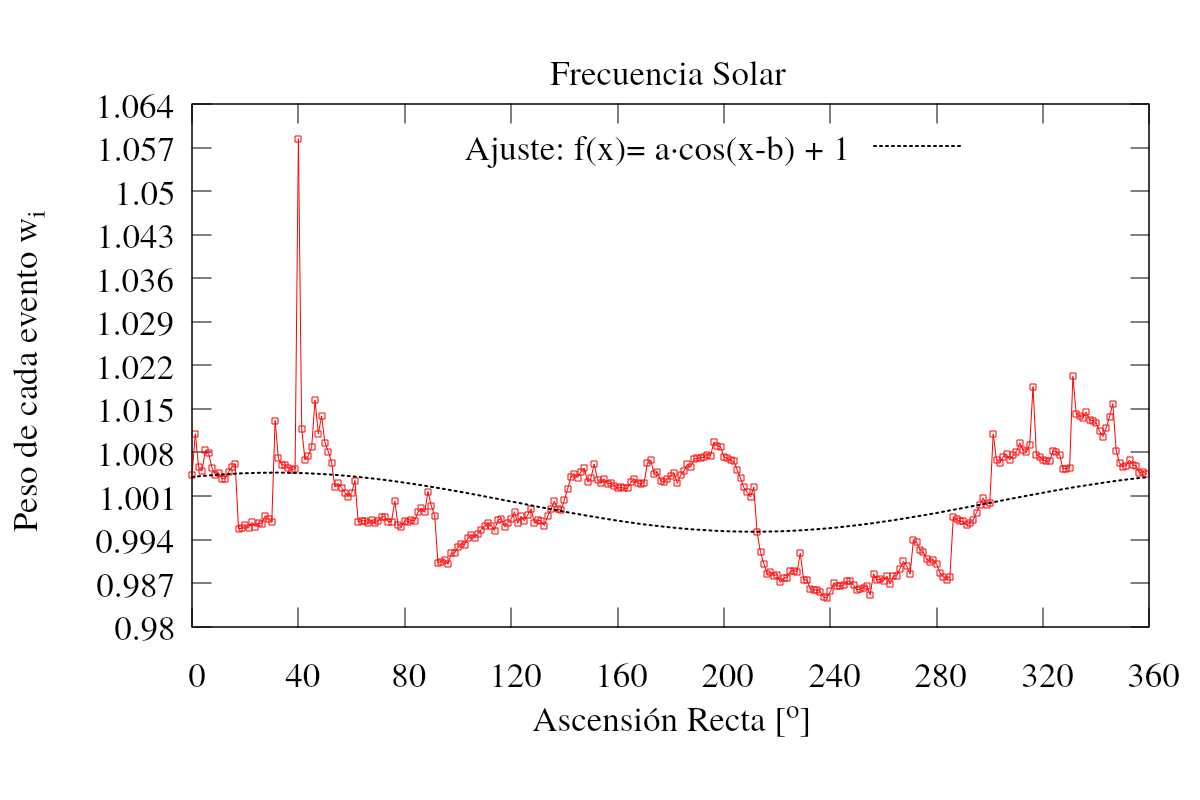
\includegraphics[width=\linewidth]{eventos_RA_ajuste_cos_solar_v3.png}
	\caption{Frecuencia solar}
	\label{fig:ajuste_solar}
\end{subfigure}\\
\centering
\begin{subfigure}{.5\textwidth}
	\centering
	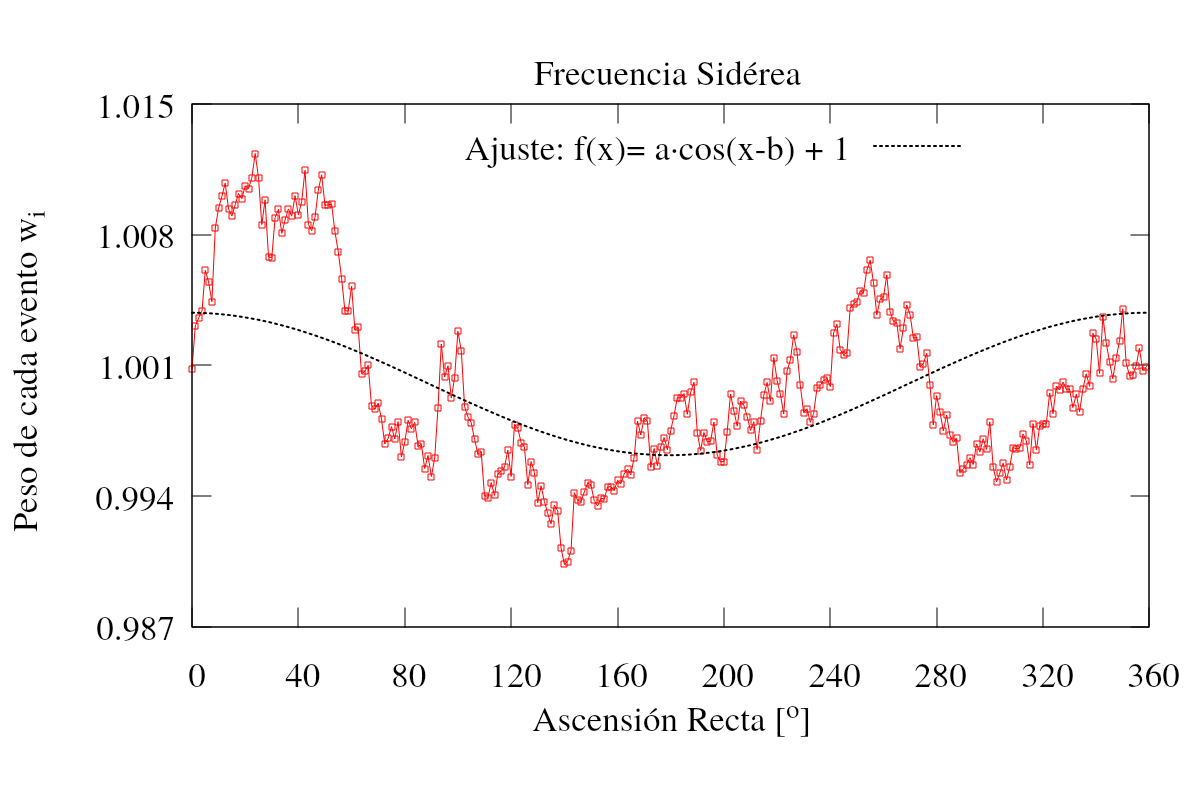
\includegraphics[width=\linewidth]{eventos_RA_ajuste_cos_siderea_v2.png}
	\caption{Frecuencia sidérea}
	\label{fig:ajuste_siderea}
\end{subfigure}%
\caption{Ajuste de los pesos de los eventos para varias frecuencias a primer orden en ascensión recta}
\end{figure}

	
\subsection{Tabla comparando los ajustes:}
		
		\begin{table}[H]
		\centering
		\begin{tabular}{c|c|c|c}
					& Anti-sidérea			& Solar 				& Sidérea\\ \hline
		Amplitud $a$& $0.0109\pm 0.0003 $ 	&	$0.0038 \pm 0.0003$	&  $0.0047\pm 0.0007$		\\
		Fase $\phi$ & $15    \pm 1$ 		&   $360 \pm 5   $ 		&  $31    \pm 8    $ 		\\
		\end{tabular}
		\caption{Parámetros obtenidos del ajuste a primer orden en $\alpha$ sobre los pesos.}
		\end{table}


\section{Gráfico de la anisotropía}
		
	\subsubsection{Análisis de anisotropías en ascensión recta}
		
		\begin{figure}[H]
			\centering
			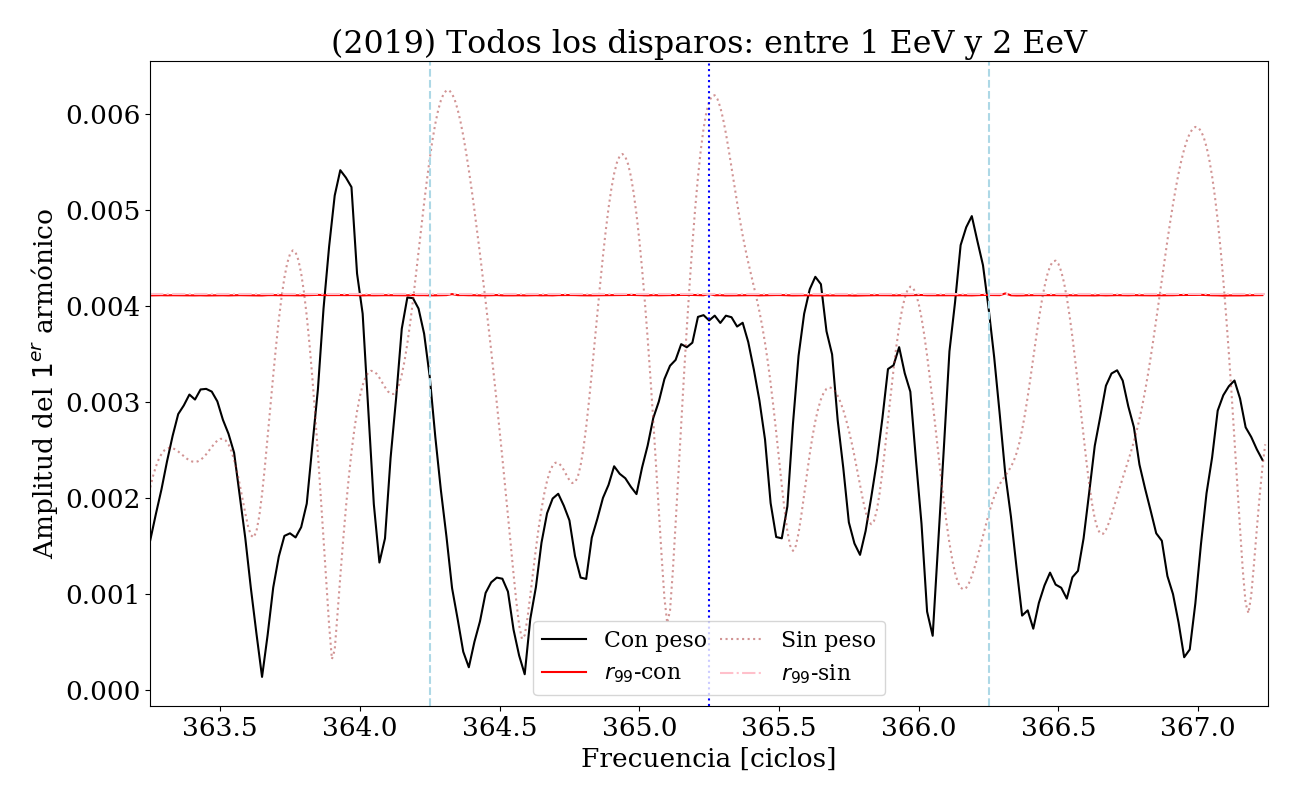
\includegraphics[width=\linewidth]{pesos_sin_con_1_2_EeV.png}
			\caption{Anisotropía en función de la frecuencia, se comparan los análisis sin los pesos y con los pesos de los hexágonos}
		\end{figure}
		
		
		\begin{table}[H]
		\centering
		\begin{tabular}{c|c|c|c|c|c}
					& Solar (sin peso)	& Solar (con peso)	&& Sidérea (sin peso) 	& Sidérea (con peso)	 \\ \hline
		Fase $\phi$ & 251	    		& 288	    		&& 289				& 335				\\
		Amplitud $r$& 0.0061	    	& 0.0038	  		&&0.0018		& 0.0039			\\
		\end{tabular}
		\caption{Comparación de los parámetros de fase y amplitud para las frecuencias sidérea y solar, analizando sin pesos y con los pesos de los hexágonos con el análisis de Rayleigh}
		\end{table}


\subsubsection{Bineado de eventos }


Considerando que estamos trabajando con la frecuencia solar al hacer el análisis con pesos, se obtiene la siguiente distribución de eventos en función de su ascensión recta.
\begin{figure}[H]
	\centering
	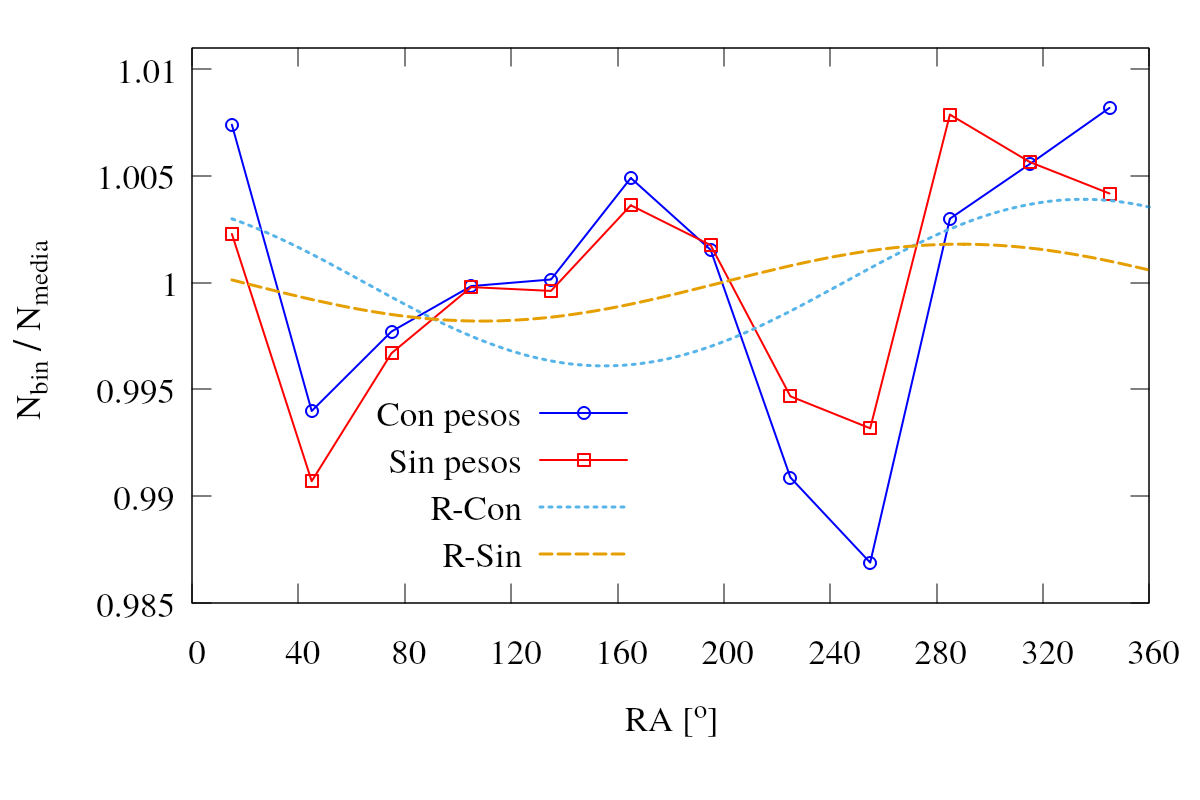
\includegraphics[width=\linewidth]{eventos_clasificados_por_RA_v4.png}
	\caption{Distribución de la cantidad relativa de eventos en función de la ascensión recta.}
\end{figure}

% Si realizamos un ajuste de una función del tipo $f(x) = a\cdot\cos{(x - \phi)}) + 1 $, se obtiene los siguientes valores
		
% 	Fase $\phi$ : $288(60)^o$  \\
% 	Amplitud $a$: 0.002(2)  	\\

